\documentclass{article}
\usepackage[utf8]{inputenc}
\usepackage[a4paper, portrait, margin=1in]{geometry}
\usepackage{graphicx}
\usepackage{subcaption}
\usepackage{tabularx}
\usepackage{hyperref}
\hypersetup{
    colorlinks=true,
    linkcolor=blue,
    filecolor=magenta,      
    urlcolor=cyan,
}
\usepackage{amsmath}

\title{Cloud Computing (UE18CS352) \\Unit 3}
\author{Aronya Baksy}
\date{March 2021}

\begin{document}

\maketitle
\section{Introduction: Disk Storage Fundamentals}
\begin{itemize}
    \item Disk latency has the following three components:
    \begin{enumerate}
        \item \textbf{Seek Time}: The time needed for the controller to position the disk head to the correct cylinder of the disk
        
        \item \textbf{Rotational Latency}: The time needed for the first sector of the block to position itself under the disk head
        
        \item \textbf{Transfer Time}: Time needed for the disk controller to read/write all the sectors on the disk. 
    \end{enumerate}
    
    \item RAID (Redundant Array of Independent Disks) is a storage virtualization technology that combines multiple physical disks into one or more logical volumes for increased redundancy and faster performance. 
    
    \item The driving technologies behind RAID are \textbf{striping},\textbf{mirroring} and \textbf{parity checking}.
\end{itemize}

\subsection{Storage Architectures}
\begin{itemize}
    \item In \textbf{Directly Attached Storage} (DAS), the digital storage is directly attached to the network node that is accessing that storage. 
    
    \item DAS is only accessible from the node to which the storage device is attached physically. 
    
    \item \textbf{Network Attached Storage} (NAS) is a file-level storage device connected to a heterogeneous group of clients. 
    
    \item A single NAS device containing physical storage devices (these may be arranged in RAID) serves all file requests from any client in the connected network. 
    
    \item NAS removes the responsibility of file serving from other servers on the network. Data is transferred over Ethernet using TCP/IP protocol. 
    
    \item \textbf{Storage Area Network} (SAN) is a network that provides access to block-level data storage. 
    
    \item  A SAN is built from a combination of servers and storage over a high speed, low latency interconnect that allows direct Fibre Channel connections from the client to the storage volume to provide the fastest possible performance.
    
    \item The SAN may also require a separate, private Ethernet network between the server and clients to keep the file request traffic out of the Fibre Channel network for even more performance. 
    
    \item It allows for simultaneous shared access, but it is more expensive than NAS and SAN. 
    
    \item  Distinct protocols were developed for SANs, such as Fibre Channel, iSCSI, Infiniband. 
\end{itemize}

\begin{figure}
    \centering
    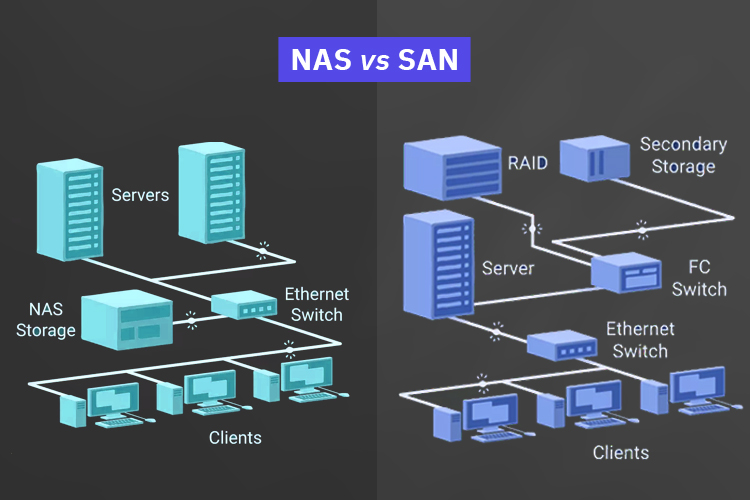
\includegraphics[scale=0.3]{nassan.jpg}
    \caption{Storage Architectures}
    \label{fig:my_label_0}
\end{figure}

\subsection{Logical Volume Management (LVM)}
\label{lvm}
\begin{itemize}
    \item LVM is a file-system virtualization layer 
    
    \item LVM provides a method of allocating space on mass-storage devices that is more flexible than conventional partitioning schemes to store volumes.
    
    \item The components of LVM are:
    \begin{enumerate}
        \item Extend volumes while a volume is active and has a full file system (shrinking volumes requires unmounting and suitable storage requirements)
        
        \item Collect multiple pysical drives into a volume group 
    \end{enumerate}
    
    \item LVM consists of the following basic components layered on top of each other:
    \begin{itemize}
        \item A \textit{physical volume} corresponds to a physical disk that is detected by the OS (labelled often as \texttt{sda} or \texttt{sdb}) (NOTE: partitions of a single actual disk are detected as separate disks by the OS). 
        
        \item A \textit{volume group} groups together one or more physical volumes
        
        \item A \textit{logical volume} is a logical partition of the volume group. Each logical volume runs a file system. 
    \end{itemize}
    
    \item The \texttt{/boot} partition cannot be included in LVM as GRUB (the GNU Bootloader that loads the bootstrap program from the master boot record) cannot read LVM metadata. 
    
\end{itemize}

\begin{figure}[!ht]
    \centering
    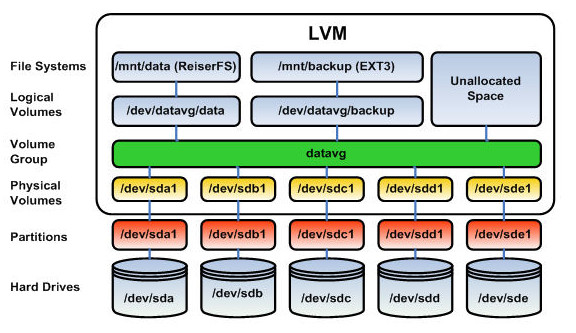
\includegraphics[scale=0.7]{LogicalVolumenManager.jpg}
    \caption{Logical Volume Management}
    \label{fig:my_label}
\end{figure}

\section{Storage Virtualization}
\begin{itemize}
    \item Abstraction of physical storage devices into logical entities presented to the user, hiding the underlying hardware complexity and access functionality (either direct access or network access)
    
    \item Advantages of storage virtualization are:
    \begin{itemize}
        \item Enables higher resource usage by aggregating multiple heterogeneous devices into pools
        
        \item Easy centralized management, provisioning of storage as per application needs (performance and cost).  
    \end{itemize}
\end{itemize}

\subsection{File-Level Virtualization}
\begin{itemize}
    \item An abstraction layer exists between client and server. 
    
    \item This virtualization layer manages files, directories or file systems across multiple servers and allows administrators to present users with a single logical file system
    
    \item Normally implemented as a network file system that has 
    \begin{itemize}
        \item Standard protocol for file sharing
        
        \item Multiple file servers enable access to files 
    \end{itemize}
    
    \item NFS, CIFS, and Web interfaces like HTTP/HTTPS are examples of this.
\end{itemize}

\subsubsection{Distributed File System}
\begin{itemize}
    \item DFS is a type of network file system that is spread across multiple interconnected nodes. 
    
    \item The objective of DFS is to enable file directory \textit{replication} (for fault tolerance) and\textit{ location transparency} (using names to refer to resources rather than their actual location)
    
    \item Recently accessed disk blocks can be cached for better performance. 
    
    \item Metadata managment is important for performance reasons. It can be either \textbf{centralized} or \textbf{distributed}
\end{itemize}

\subsubsection{DFS with centralized metadata: Lustre}
\begin{itemize}
    \item All metadata operations by clients are directed to a single dedicated metadata server. 
    
    \item Lock-based synchronization is used in every read or write operation from the clients.
    
    \item When workloads involve large files, such systems scale well. But the metadata server can become a SPOF or a performance bottleneck when loads increase. 
    
    \item \textbf{Lustre} is a massively parallel, scalable distributed file system for Linux that uses DFS with centralized metadata. 
    
    \item It is available under GNU General Public License, and used on many supercomputer grids that run Linux. 
    
    \item The components of Lustre are:
    \begin{enumerate}
        \item \textbf{ Object Storage Server} (OSS), store file data on object storage targets (OSTs). A single OSS can serve 2-8 OSTs. The total capacity of a Lustre FS is the sum of capacities provided by the OSS across all the OST nodes. 
        
        \item \textbf{Metadata target} (MDT) stores metadata on one or more metadata servers (MDS)
        
        \item \textbf{Luster clients} access data over a network using a POSIX-compliant interface. 
    \end{enumerate}
    
    \item The file access is done in the following sequence:
    \begin{itemize}
        \item Client performs a lookup on the MDS for a filename. 
        
        \item MDS either returns layout for the existing file, or creates the metadata for a new file. 
        
        \item The client passes this layout to a Logical Object Volume (LOV). The LOV maps the layout to objects and their actual locations on different OSTs
        
        \item The client then locks the file range being operated on and executes one or more parallel reads/writes directly to the OSTs
    \end{itemize}
\end{itemize}

\subsubsection{DFS with distributed metadata : Gluster}
\begin{itemize}
    \item Metadata distributed among all the network nodes. Involves greater complexity as metadata has to be managed across multiple nodes
    
    \item \textbf{Gluster} is an open-source distributed file system with distributed metadata. It is optimized for high performance, and scales up to 1000s of clients and PB of data. 
    
    \item Gluster mploys a modular architecture with a stackable user-space design. 
    
    \item It aggregates multiple \textbf{storage bricks} on a network (over Infiniband RDMA or TCP/IP interconnects) and delivers as a network file system with a global name space
    
    \item The components of Gluster are:
    \begin{itemize}
        \item \textbf{Server} delivers the combined disk space of all the physical storage servers as a single file system
        
        \item \textbf{Client} implements highly available, massively parallel access to each storage node along with node failure handling 
    \end{itemize}
    
    \item A storage brick is a server (containing directly attached storage or connected to a SAN) on which a file system (like ext3 or ext4) is created 
    
    \item A translator is a layer between a brick and the actual user. It acts as a file system interface and implements one single Gluster functionality
    
    \item I/O Scheduling Translators are responsible for load balancing,
    
    \item Automatic File Replication (AFR) translator keeps identical copies of a file/directory on all its subvolumes (used for replication)
\end{itemize}

\subsection{Block-Level Virtualization}
\begin{itemize}
    \item Virtualizes multiple physical disks into a single virtual disk
    
    \item Data blocks are mapped to one or more physical disks sub-systems. 
\end{itemize}

\subsubsection{Host-based BLV}
\begin{itemize}
    \item Uses LVM (section \ref{lvm}) to support dynamic resizing of volumes, or combine fragments of unused disk space into a single volume, or create virtual disks (with size larger than physical disk)
\end{itemize}

\subsubsection{Storage Device-level BLV}
\begin{itemize}
    \item Creates Virtual Volumes over the physical storage space of the specific storage subsystem.
    
    \item Using RAID techniques, logical units are created that span mulitple disks. 
    
    \item Host independent and low latency as virtualization is built into the firmware and hardware of the storage device
\end{itemize}

\subsubsection{Network-Level BLV}
\begin{itemize}
    \item Most commonly implemented, scalable form, implemented as part of the interconnect network between storage and hosts (e.g.: Fibre Channel SAN)
    
    \item \textbf{Switch-based}: the actual virtualization occurs in an intelligent switch in the network, and it works in conjunction with a metadata manager
    
    \item \textbf{Appliance-based}: I/O is routed through an appliance that manages the virtualization layer
    
    \item \textbf{In-band appliances} perform all I/O with zero direct interaction between client and storage. 
    
    \item \textbf{Out-of-band appliances} manage only metadata (control paths) while the actual data flows directly between client and storage server (each client having an agent to manage this)
\end{itemize}

\section{Object Storage Technologies}
\subsection{Amazon Simple Storage Service (S3)}
\begin{itemize}
    \item Highly reliable, available, scalable, fast cloud storage that supports storage and retrieval of large amounts of data using simple web services
    
    \item Interaction with S3 is done via the GUI (Amazon Console), the TUI (Amazon CLI) or language specific abstractions. A RESTful API is provided for basic HTTP operations
    
    \item Files are called \textbf{objects}. The \textbf{key} of an object is its identification (directory path + object name). All objects are stored in \textbf{buckets}.
    
    \item S3 objects are replicated across multiple global zones. Versioning enables further recovery from modification and deletion by accident.
    
    \item Security is maintained in S3 using:
    \begin{itemize}
        \item \textbf{Access Control Lists}: Set permissions to allow other users to access an object
        
        \item \textbf{Audit Logs}: Once enabled, stores the access log for an bucket. This enables one to identify the AWS account, IP Address, time of access and operations performed by the one who accessed. 
    \end{itemize}
    
    \item Data Security is maintained in S3 using:
    \begin{itemize}
        \item \textbf{Replication}: across multiple devices, allows for upto 2 replica failures (cheaper option is Reduced Redundancy Storage which survives only 1 replica failure), but consistency across replicas is \textit{not guaranteed}.
        
        \item \textbf{Versioning}: If enabled, S3 stores the full history of each object. It allows for changes to be undone, including file deletions.
        
        \item \textbf{Regions}: select location of S3 bucket for performance/legal reasons. 
    \end{itemize}
    
    \item S3 allows for large objects to be uploaded in parts. These parts can be uploaded in parallel for maximum network utilization
\end{itemize}

\subsection{DynamoDB - NoSQL Service}
\begin{itemize}
    \item Cloud-based NoSQL database that is available with AWS. Consists of tables created and defined in advance (with some dynamic elements)
    
    \item Overall is schemaless.
    
    \item Supports only item-level consistency (similar to row-level consistency in RDBMS). If cross-item consistency is needed then don't use DynamoDB
    
    \item Joins are implemented only at the applicaiton side. DynamoDB \textit{does not support joins} between tables. 
    
    \item Table is collection of items, item is collection of attribute-value pairs. Primary key identifies items uniquely in a table.
    
    \item A partition is an allocation of storage for a table, backed by SSDs and automatically replicated across multiple Availability Zones within an AWS Region. 
    
    \item Types of primary keys in DynamoDB:
    \begin{itemize}
        \item \textbf{Partition Key}: The value of the partition key attribute is passed into a hash function to determine the physical partition on which that item will be stored
        
        \item \textbf{Partition + Sort Keys}:  All items with the same partition key hash value are stored together in sorted order by sort key value.  
    \end{itemize}
    
    \item Users can also create secondary keys in addition to primary keys for alternate queries.
\end{itemize}

\subsection{Amazon Relational DB Service (RDS)}
\begin{itemize}
    \item Provides an abstraction of an RDBMS. Offers all majorly used RDBMS such as Amazon Aurora, PostgreSQL, MySQL, Oracle, MS SQL Server
    
    \item AWS performs all admin tasks related to maintenance, as well as periodic backups of the DB state and the ability to take snapshots. 
    
    \item RDS provides encryption at rest and in transit, as well as APIs for applications. 
\end{itemize}

\section{Partitioning}
\begin{itemize}
    \item Breaking down large DBs into smaller units that are stored on different machines. Each row belongs to exactly one partition
    
    \item Supports operations that touch mulitple partitions at the same time. 
    
    \item Motivation is \textbf{scalability} in terms of load balancing and query throughput, as well as fault tolerance (when combined with replication)
    
    \item Small queries can be independently processed by one partition. Large queries can be parallelized between multiple partitions. 
    
    \item When some partitions have more data than others, they are said to be \textbf{skewed}. A partition with disproportionately high load is called a \textbf{hot spot}
\end{itemize}

\subsection{Partitioning Strategies}
\subsubsection{Randomized Partitioning}
\begin{itemize}
    \item Distribute the data quite evenly across the nodes
    
    \item Disadvantage: When trying to read a particular item, no way of knowing which node it is on, so all nodes need to be queried in parallel. 
\end{itemize}

\subsubsection{Partitioning by Key Range}
\begin{itemize}
    \item Assign range of key values to a given partition. If partition boundaries are known then determining which partition a given key is in is very simple
    
    \item Ranges may not be equal width, as data distribution is not uniform
    
    \item Each partition can have keys in sorted order
    
    \item Disadvantage: certain access patterns can lead to hot spots (e.g.: storing sensor data, if the key is timestamp then all writes go to one single partition which the current day's partition)
\end{itemize}

\subsubsection{Partitioning by Hash of Key}
\begin{itemize}
    \item Using a suitable hash function for keys, each partition has a range of hash values assigned to it (rather than a range of keys), and every key whose hash falls within a partition’s range will be stored in that partition.
    
    \item A good hash function takes skewed data and makes it uniformly distributed
    
    \item Simple hash partitioning do not allow efficient range queries. This is solved using composite keys. 
    
    \item \textbf{Consistent hashing} is a way of evenly distributing load across an internet-wide system of servers such as a content delivery network
    
    \item It uses randomly chosen partition boundaries to avoid the need for central control or distributed consensus
\end{itemize}

\subsection{Secondary Indexes}
\begin{itemize}
    \item Do not map neatly to partitions, but useful for increasing performance of queries made on a particular key.
\end{itemize}

\subsubsection{Document-based Secondary Indexing}
\begin{itemize}
    \item Also called \textbf{local secondary indexing}
    
    \item Each partition maintains its own secondary index, covering only the documents in that partition. 
    
    \item Reading involves reading from each and every partition and separately combining the results. This approach is called \textbf{scatter-gather}, and it makes read queries expensive
    
    \item Even if the partitions are queried in parallel, scatter/gather is prone to tail latency amplification
\end{itemize}

\subsubsection{Term-based Secondary Indexing}
\begin{itemize}
    \item A single \textbf{global secondary index} covers data from all partitions. 
    
    \item The index is stored on multiple nodes, partitioned by the term (for range scans) directly, or a hash of the term (for load balancing)
    
    \item Reads are more efficient as a query is made only to the partition where the term resides
    
    \item Writes are less efficient as a write affects multiple partitions of the index. This requires a distributed transaction across all partitions affected by a write
    
    \item In practice, updates to global secondary indexes are often asynchronous
\end{itemize}

\subsection{Rebalancing Partitions}
\begin{itemize}
    \item The process of moving load from one node in the cluster to another is called rebalancing.
    
    \item Requirements of rebalancing:
    \begin{itemize}
        \item After rebalancing, loads should be shared fairly between all cluster nodes 
        
        \item During rebalancing the system should still accept read/write requests
        
        \item Minimize the amount of data moved around to reduce network and I/O overheads

    \end{itemize}
    
    \item The following are rebalancing strategies:
\end{itemize}

\subsubsection{Hash mod n}
\begin{itemize}
    \item hash(key) \% n returns a number between 0 and n-1, corresponding to a single partition
    
    \item Simple, but drawback is that any change in N leads to rehashing of large number of keys which makes the rebalancing very expensive
\end{itemize}

\subsubsection{Fixed number of partitions}
\begin{itemize}
    \item Move only entire partitions. Assignment of keys to partitions does not change, but only assignment of partitions to nodes changes.
    
    \item Create many more partitions than there are nodes and assign several partitions to each node
    
    \item  If a node is added to the cluster, the new node can steal a few partitions from every existing node until partitions are fairly distributed once again
    
    \item So many fixed-partition databases choose not to implement partition split and merge 
    
    \item Choosing the right number of partitions is difficult if the size of the dataset is variable
\end{itemize}

\subsubsection{Dynamic Partitioning}
\begin{itemize}
    \item Fixed number of partitions can become imbalanced as data is inserted and removed from the database
    
    \item In dynamic partitioning, the number of partitions adapts to the total data volume
    
    \item In dynamic partitioning, the partitions split if they grow beyond an upper bound. If the partition shrinks below a lower bound, it can be merged with an adjacent partition
    
    \item Can be used with both key-range partitioned and hash partitioned data
\end{itemize}

\subsubsection{Proportional to number of nodes}
\begin{itemize}
    \item The size of each partition grows proportionally to the dataset size while the number of nodes remains unchanged, but when number of nodes increase, the partitions become smaller again
    
    \item Keeps partition sizes stable
    
    \item When a new node joins the cluster, it randomly chooses a fixed number of existing partitions to split, and then takes over half of each of those split partitions. 
\end{itemize}

\subsection{Request Routing}
\begin{itemize}
    \item In case of a dataset partitioned among multiple nodes, which node should read/write requests from a client go to? Request routing solves this issue
    
    \item Approaches to routing are:
    \begin{itemize}
        \item Client contacts one node at random. If that node contains the request partition then it serves the client, else it forwards the request to the appropriate node (this requires all nodes to be aware of partition -$>$ node assignments)
        
        \item Client contacts a routing tier, which is aware of all the node assignments. It forwards the request to the appropriate node. The routing tier only acts as a \textit{partition-aware load balancer}
        
        \item Client directly contacts the appropriate node on which the requested partition lies, requiring each client to know about partitioning and assignment to nodes. 
    \end{itemize}
\end{itemize}

\subsubsection{ZooKeeper}
\begin{itemize}
    \item A distributed metadata management system for clusters. 
    
    \item ZooKeeper maintains an authoritative mapping between partititons and nodes, and each node registers itself with the ZooKeeper service. 
    
    \item Other actors, such as the routing tier or the partitioning-aware client, can subscribe to this information in ZooKeeper
    
    \item When partitioning changes or node removal/addition occurs, ZooKeeper notifies the routing tier 
\end{itemize}

\section{Replication}
\begin{itemize}
    \item Keeping multiple copies of a single partition on different nodes connected by a network
    
    \item Motivation for replication:
    \begin{itemize}
        \item Reduce latency by reducing distance to user
        
        \item Increase availability by allowing fault tolerance
        
        \item Increase read throughput by allowing more parallel reads (scalable)
    \end{itemize}
\end{itemize}

\subsection{Single Leader Replication}
\begin{itemize}
    \item Among all replicas, elect one leader and keep all other partitions as followers.
    
    \item All write requests from clients are directed to the leader, but read requests can be served by leader or followers
    
    \item When a leader gets a read request, it first updates its own write log. This write log is transmitted to all the followers, and the followers apply the changes in the same order as the leader. 
    
    \item In \textbf{synchronous replication}, the leader waits for all followers to confirm that they have received a write request, and only then sends success message to the user. 
    
    \item In \textbf{asynchronous replication}, the leader sends the success message to the user without waiting for followers to acknowledge the receipt of the write. 
    
    \item In \textbf{semi-synchronous replication}, the leader waits for exactly one follower to confirm that it has received a write request, and only then sends success message to the user. 
    
    \item Sychronous replication sacrifices availability for consistency, vice versa for asynchronous
\end{itemize}

\subsubsection{Node Failure}
\begin{itemize}
    \item Follower failure is handled using \textbf{catch-up recovery}. Follower stores the edit logs on its disk
    
    \item If a failed follower is restarted, then it can ask the leader for all log entries between the time it crashed and the current time. Upon receiving this, the follower replayed these log entries to get the updated data
    
    \item In case of leader failure, one of the old followers has to be elected to the position of leader. Clients are to be reconfigured to send their write queries to this new leader
    
    \item Leader failover takes place manually (by theactions of a system admin) or automatically. The steps in leader failover are:
    \begin{itemize}
        \item Identify leader failure
        
        \item Elect a new leader
        
        \item Reconfigure system to use the new leader
    \end{itemize}
\end{itemize}

\subsubsection{Implementation}
\begin{itemize}
    \item \textbf{Statement Replication}: The leader logs every write request that it executes and sends that statement log to its followers (fails for non-deterministic functions like \texttt{rand()} and \texttt{now()})
    
    \item \textbf{Write-Ahead Log Shipping}: The leader writes the log (an append-only byte stream) to disk and sends it across the network to its followers. When the follower processes this log, it builds a copy of the exact same data structures as found on the leader.
    
    \item \textbf{Logical Log Replication}: Uses different log formats for replication and for the storage engine. A logical log (aka the replication log) is a sequence of records describing writes to database tables at the row level
    
    \item \textbf{Trigger-Based Replication}: A trigger on the leader table logs the change to another table where an external process can read it. The external process applies the replication to another system
\end{itemize}

\subsection{Replication lag}
\begin{itemize}
    \item The delay between a write happening on the leader and the same being reflected on a follower is known as the replication lag.
    
    \item Read-After-Write consistency is a guarantee for a \textit{single user}, in that if the same user reads the data at any time interval after reading it, the user will get the updated data. 
    
    \item Solutions:
    \begin{itemize}
        \item Read critical data from leader, rest from follower (negates scaling advantage)
        
        \item Prevent queries on any follower that is lagging significantly behind the leader 
        
        \item Client remembers the timestamp of their most recent write, and ensure that the node serving that user is updated atleast till that timestamp
        
        \item Monotonic reads: each user read from the same replica always
        
        \item Consistent prefix reads - if a sequence of writes happen in a certain order, then anyone reading those writes should see them appear in the same order
    \end{itemize}
\end{itemize}

\subsection{Multi-Leader Replication}
\begin{itemize}
    \item Allow more scalability in writes by allowing multiple leaders. Each leader simultaneously acts as a follower to the other leaders.
    
    \item Conflict Avoidance:
    \begin{itemize}
        \item Ensure that all writes for a particular record go through the same leader
        
        \item Give each write an unique ID and pick the write with the highest ID (throw the others away)
        
        \item Custom conflict resolution logic in the application code that  may be executed on write/reads
    \end{itemize}
    
    \item In a multi leader config, the writes can go to the nearest leader only and replicated asynchronously to all the other leaders (better perceived performance)
    
    \item In a single leader config, the failure of a leader means there is downtime involved in failover. 
    
    \item In a multi-leader config, each datacenter can continue operating independently of the others, and replication catches up when the failed datacenter is back online. 
    
    \item In a single-leader config, the public internet is used for synchronous updates between leader and follower, hence is sensitive to problems in this network
    
    \item A multi-leader config with asynchronous replication tolerates network problems better as a temporary network problems do not prevent writes being processed
\end{itemize}

\subsection{Leaderless Replication}
\begin{itemize}
    \item No single dedicated leader, all replicas of a partition are the same from the client point of view.
    
    \item In some implementations, the client sends writes to multiple nodes at the same time
    
    \item In others, a single co-ordinator node does this on behalf of the client, but it does not enforce a particular order of writes (like a leader in a single-leader set up does)
    
    \item If writes are sent to multiple nodes, but some nodes out of these fail and hence cannot complete the write. If the nodes that failed come back online, then any data on them is now out of date (stale)
    
    \item To solve this issue, each data item has a version number associated with it. The client reading from multiple replicas checks the version number of the data and selects the most recent one. 
    
    \item When the client reads values with different version numbers, the client writes the most recent version of the data to all the nodes with less recent versions. This is called \textbf{read repair}
    
    \item A background process (rather than the client itself) monitors all data values and their versions across all nodes, and periodically writes the latest value of the data to all the replicas. This is called an \textbf{anti-entropy process}.
    
    \item Let there be $n$ nodes. Let $r$ nodes be queried for each read, and $w$ nodes confirm for each write. If 
    \begin{equation*}
        w + r > n
    \end{equation*}
    then an up-to-date copy of the data is guaranteed while reading, as at least one of the $r$ nodes being read from must be up to date.
    
    \item Reads and writes that obey the above rule are called \textbf{quorum reads and writes}. 
\end{itemize}

\subsubsection{Monitoring}
\begin{itemize}
    \item Monitoring in leaderless systems is difficult as writes do not happen in any particular order 
    
    \item In single-leader systems, the writes are in a fixed order maintained on the edit log of the leader. The out-of-date follower can compare its position (timestamp) with that of the leader and make the necessary changes.
\end{itemize}

\subsubsection{Multi-datacenter Operation}
\begin{itemize}
    \item Leaderless replication is suitable for multi-datacenter operation, since it is designed to tolerate conflicting concurrent writes, network interruptions and latency spikes.
    
    \item The number of replicas of a single partition $n$ is across all datacenters. Number of replicas in a single datacenter can be configured
    
    \item All writes are sent to all replicas, but only a quorum of nodes within the local datacenter is sufficient for the client to detect a success. 
    
    \item The higher-latency writes to other datacenters are often configured to happen asynchronously
\end{itemize}

\subsubsection{Detecting concurrent writes}
\begin{itemize}
    \item Several clients writing to the same key concurrently means that conflicts will occur (even if quorum is followed)
    
    \item Events may arrive in a different order at different nodes, due to variable network delays and partial failures
    
    \item \textbf{Last Write Wins}: each replica stores the value with the highest version number only (discarding the rest of the data)
    
    \item Given two events $A$ and $B$, $A$ is said to \textbf{happen before} $B$ if $B$ knows about $A$, or depends on $A$ or builds on $A$. 
    
    \item Definition of concurrency is dependent on this happens-before relationship. Server can determine whether two operations are concurrent by looking at the version numbers
\end{itemize}

\subsubsection{Algorithm for detecting concurrent operations}
\begin{itemize}
    \item A client must read a key before writing to it.
    
    \item When a client reads a key, the replica sends the values that have not been overwritten, as well as the latest version number
    
    \item When a client writes a key, it must include the version number from the prior read, and it must merge together all values that it received in the prior read.
    
    \item When the server receives a write with a particular version number, it can overwrite all values with that version number or below, but still maintains the values with higher version numbers. 
    
    \item The collection of all version numbers for an item across all its replicas is called the \textit{version vector}
    
    \item Version vectors are sent from the database replicas to clients when values are read, and need to be sent back to the database when a value is subsequently written
    
    \item The version vector allows the database to distinguish between overwrites and concurrent writes, and ensures that it is safe to read from one replica and write to another. 
\end{itemize}

\section{Consistency Models}
\begin{itemize}
    \item Most distributed systems only guarantee \textbf{eventual consistency} 
    \item In eventual consistency, data read at any point may not be consistent across nodes, but if there are no writes for some unspecified interval then all the nodes can catch up to the consistent state
    
    \item This is a weak guarantee, as it does not give any guarantees about actual time of consistency. 
\end{itemize}
\subsection{Linearizability}
\begin{itemize}
    \item The illusion that there is only one copy of a data item across a distributed system. (implies that all data must be up to date at all times, no staleness in caching)
    
    \item Ensures that applications running on the distributed system do not need to worry about replication. 
    
    \item Main point of linearizability: After any one read has returned the new value, all following reads (on the same or other clients) must also return the new value.
    
    \item \textbf{Compare-and-Set} is an operation on the database:
    \begin{itemize}
        \item The CAS operation takes in 3 arguments: a memory location to read from (called $X$), an old value ($v_{old}$) and a new value ($v_{new}$)
        
        \item If $X == v_{old}$ then set $X := v_{new}$
        
        \item If $X \ne v_{old}$ then return an error, don't change the value in $X$
    \end{itemize}
    
    \item Test for linearizable behaviour: record the timings of all requests and responses and check whether a valid sequential ordering can be constructed from them. 
    
    \item In synchronous mode, single leader replication is linearizable. 
    
    \item Consensus algorithms implement measures to avoid stale replicas, and implement safe linearizable storage. (e.g.: ZooKeeper)
    
    \item Multi-leader and leaderless replication are not linearizable (leaderless probably not)
\end{itemize}

\subsection{CAP Theorem}
\begin{itemize}
    \item \textbf{Consistency} requires that all reads after a write return the same value, which is the latest value
    
    \item \textbf{Availability} requires that any node (that is not in a failure state) is ready to process requests. 
    
    \item \textbf{Partition Tolerance} requires that a system is tolerant to any network or node failures by rerouting the communications.
    
    \item The CAP Theorem states that a distributed system can satisfy at most two of these 2 constraints at a time
    
    \item Consistent and Partition Tolerant systems: If a network outage causes one node to be unavailable, then such a system can still use a majority consensus and deliver consistent results (e.g.: MongoDB, Redis, BigTable)
    
    \item Available and Partition Tolerant systems: If a network outage disconnects two nodes, then they can still independently process results but there is no consistency guarantee between the data on the 2 nodes. (e.g.: Cassandra, Riak, CouchDB)
    
    \item Consistent and Available systems: Ones that cannot handle any network failures (e.g.: RDBMS such as SQL Server, MySQL)
    
    \item The modern CAP goal is to maximize combinations of consistency and availability that make sense for the specific application, while incorporating plans for unavailability and recovery of failed partitions. 
\end{itemize}

\subsection{Two Phase Commit}
\begin{itemize}
    \item Every node has a transaction \textbf{manager} that:
    \begin{itemize}
        \item Maintains transaction log for recovery
        
        \item Co-ordinates concurrent transactions at the node
    \end{itemize}
    
    \item Every node has a transaction \textbf{co-ordinator} that:
    \begin{itemize}
        \item Starts the execution of a transaction at the site, distributes the sub-transactions to other sites
        
        \item Co-ordinates the termination of the transaction (either a successful commit on all nodes or abort on all nodes)
    \end{itemize}
    
    \item A concurrency control system must:
    \begin{itemize}
        \item be resilient to node/communication link failure
        
        \item allow parallelism for greater throughput
        
        \item Optimize cost and communication delay
        
        \item Place constraints on atomic actions
    \end{itemize}
    
    \item Either commit at all sites, or abort at all sites. The 2PC mechanism is designed to implement this.
\end{itemize}

\subsubsection{Phase 1}
\begin{itemize}
    \item Coordinator places the record \textbf{Prepare T} on its log. The message is then sent to all the sites.
    
    \item Each site that receives the message decides whether to commit the componenet of transaction T or to abort it. 
    
    \item A site that wants to commit enters the pre-commit stage (in this state the site can no longer abort the transaction)
    
    \item The site takes the necessary actions to ensure that its component of T will not be aborted, then writes the log message \textbf{Ready T}. 
    
    \item Once the log is stored on disk at the site, the site sends the \textbf{Ready T} message back to the coordinator
    
    \item A site that doesn't want to commit sends the message \textbf{Don't Commit T} back to the coordinator
\end{itemize}

\subsubsection{Phase 2}
\begin{itemize}
    \item If Coordinator gets \textbf{Ready T} from all the sites, it logs the message \textbf{Commit T} and sends it to all the sites
    
    \item If the coordinator has received \textbf{don’t commit T} from one or more sites, it logs \textbf{Abort T} at its site and then sends \textbf{abort T} messages to all sites involved in T

    
    \item If a site receives a \textbf{commit T} message, it commits the component of T at that site, logging \textbf{Commit T} as it does
    
    \item If a site receives the message \textbf{Abort T}, it aborts T and writes the log record \textbf{Abort T}
\end{itemize}
\end{document}